\documentclass{beamer}
\setbeamertemplate{caption}[numbered]
\setbeamertemplate{bibliography item}[text]
\mode<presentation>{
    \usetheme{Madrid}
    \usecolortheme{beaver}
}
% \usepackage{ctex}
\usepackage{url}
\def\UrlBreaks{\do\A\do\B\do\C\do\D\do\E\do\F\do\G\do\H\do\I\do\J
\do\K\do\L\do\M\do\N\do\O\do\P\do\Q\do\R\do\S\do\T\do\U\do\V
\do\W\do\X\do\Y\do\Z\do\[\do\\\do\]\do\^\do\_\do\`\do\a\do\b
\do\c\do\d\do\e\do\f\do\g\do\h\do\i\do\j\do\k\do\l\do\m\do\n
\do\o\do\p\do\q\do\r\do\s\do\t\do\u\do\v\do\w\do\x\do\y\do\z
\do\.\do\@\do\\\do\/\do\!\do\_\do\|\do\;\do\>\do\]\do\)\do\,
\do\?\do\'\do+\do\=\do\#} 
\usepackage{graphicx}
\usepackage{booktabs}
\usepackage{ulem}
\usepackage{bookmark}
\usepackage{listings}
\usepackage{amsmath}
\usepackage{array}
\usepackage{geometry}
\title{A Synthetic Task for FGIC}
\subtitle{Main Project of Artificial Neural Network}
\author{Tianxing Yang, Zihao Liang and Haoyu Chen}
\institute{School of Computer Science and Engineering, SYSU}
\date{\today}
\begin{document}
    \begin{frame}
        \titlepage
    \end{frame}
    \begin{frame}
        \frametitle{Content}
        \tableofcontents[hideallsubsections]
    \end{frame}
    \section{Task 1\&2: Baseline and Fine-tune}
        \begin{frame}
            \frametitle{Baseline}
            \begin{itemize}
                \item Various training tricks to improve model performance
                \item Transfer learning: fine-tune pretrained model
            \end{itemize}
            Focus on Stanford Dogs dataset for this slide.\par
        \end{frame}
        \begin{frame}
            \frametitle{Training Settings}
            \begin{itemize}
                \item Using ResNet50 as main model
                \item Resize each image to $512\times512$ (keep the ratio of images by padding)
                \item Random gray scale and random flip
                \item Normalize each image by universial parameter $([0.485, 0.456, 0.406], [0.229, 0.224, 0.225])$
                \item Batch size = 16
            \end{itemize}
        \end{frame}
        \begin{frame}
            \frametitle{Training Tricks}
            \begin{itemize}
                \item Use pretrained model
                \item Using SGD as optimizer and LR scheduler
                \item learning rate=0.01, momentum=0.9, gamma=0.1
                \item Epoch num=25, LR scheduler step size=7
            \end{itemize}
        \end{frame}
        \begin{frame}
            \frametitle{Result of Baseline}
            \begin{figure}[H]
                \centering
                \begin{minipage}[t]{0.48\textwidth}
                \centering
                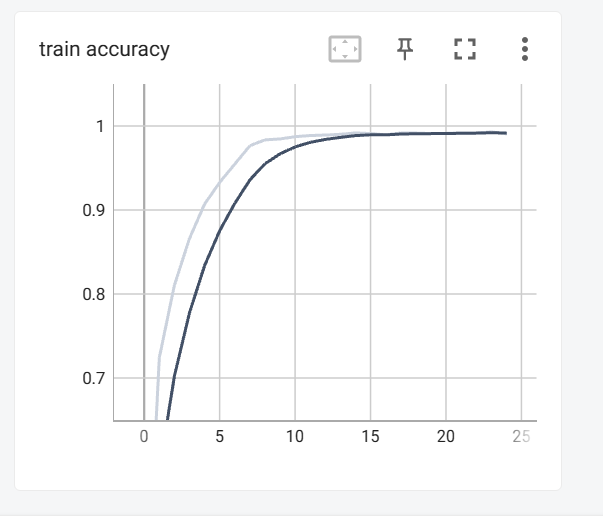
\includegraphics[width=5cm]{./img/train_acc.png}
                \caption{train-acc}
                \end{minipage}
                \begin{minipage}[t]{0.48\textwidth}
                \centering
                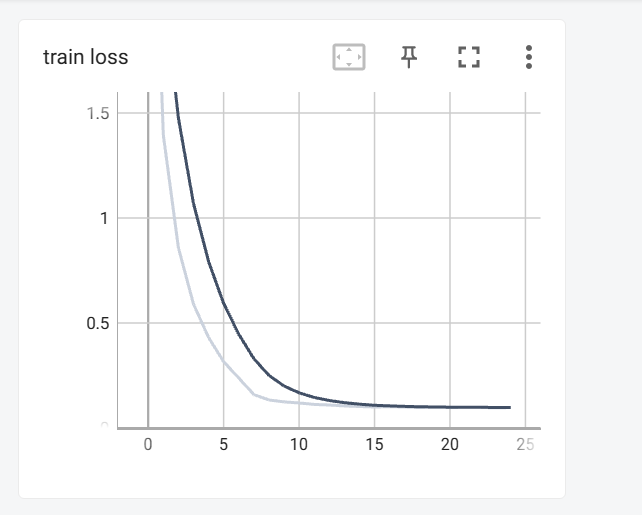
\includegraphics[width=5cm]{./img/train_loss.png}
                \caption{train-loss}
                \end{minipage}
            \end{figure}\par
        \end{frame}
        \begin{frame}
            \frametitle{Result of Baseline}
            \begin{figure}[H]
                \centering
                \begin{minipage}[t]{0.48\textwidth}
                \centering
                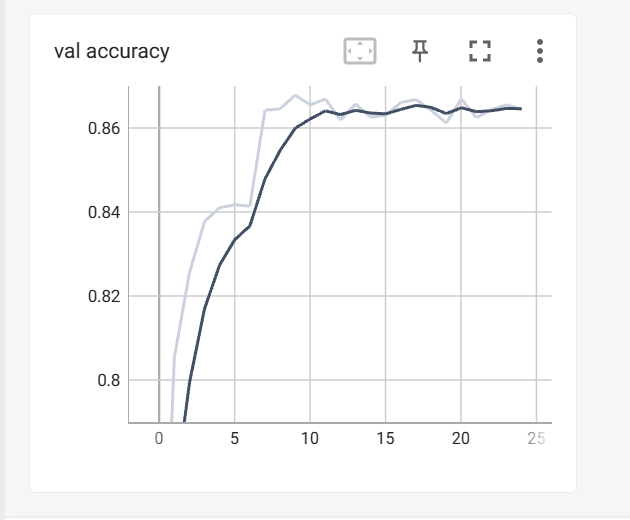
\includegraphics[width=5cm]{./img/val_acc.png}
                \caption{test-acc}
                \end{minipage}
                \begin{minipage}[t]{0.48\textwidth}
                \centering
                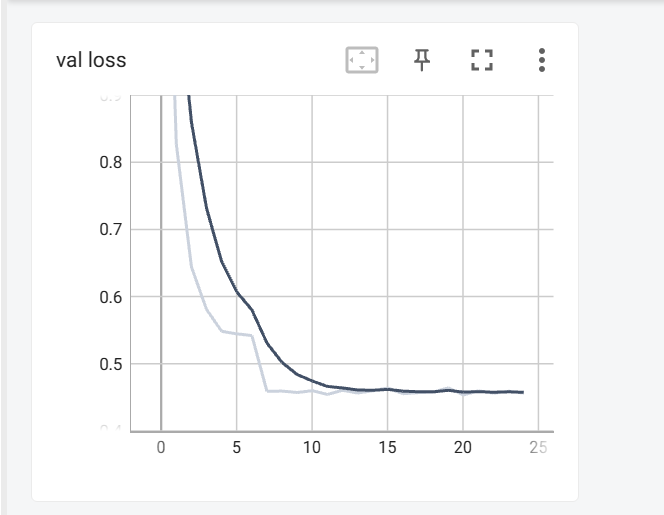
\includegraphics[width=5cm]{./img/val_loss.png}
                \caption{test-loss}
                \end{minipage}
            \end{figure}\par
        \end{frame}
    \section{Task 3: Object Detection}
        \begin{frame}
            \frametitle{Framework}
            \begin{itemize}
                \item Using MMDetection as objection framework
                \item Use sahi library to transform annnotation of Stanford Dogs dataset to COCO format
                \item Train/Inference Stanford Dogs dataset as custom dataset by using MMengine
            \end{itemize}
        \end{frame}
        \begin{frame}
            \frametitle{Object Detection}
            \begin{itemize}
                \item Training from scratch
                \item Using Faster RCNN as model
                \item Using ResNet-101 as model backbone
            \end{itemize}
        \end{frame}
        \begin{frame}
            \frametitle{Object Detection}
            \begin{figure}[H]
                \centering
                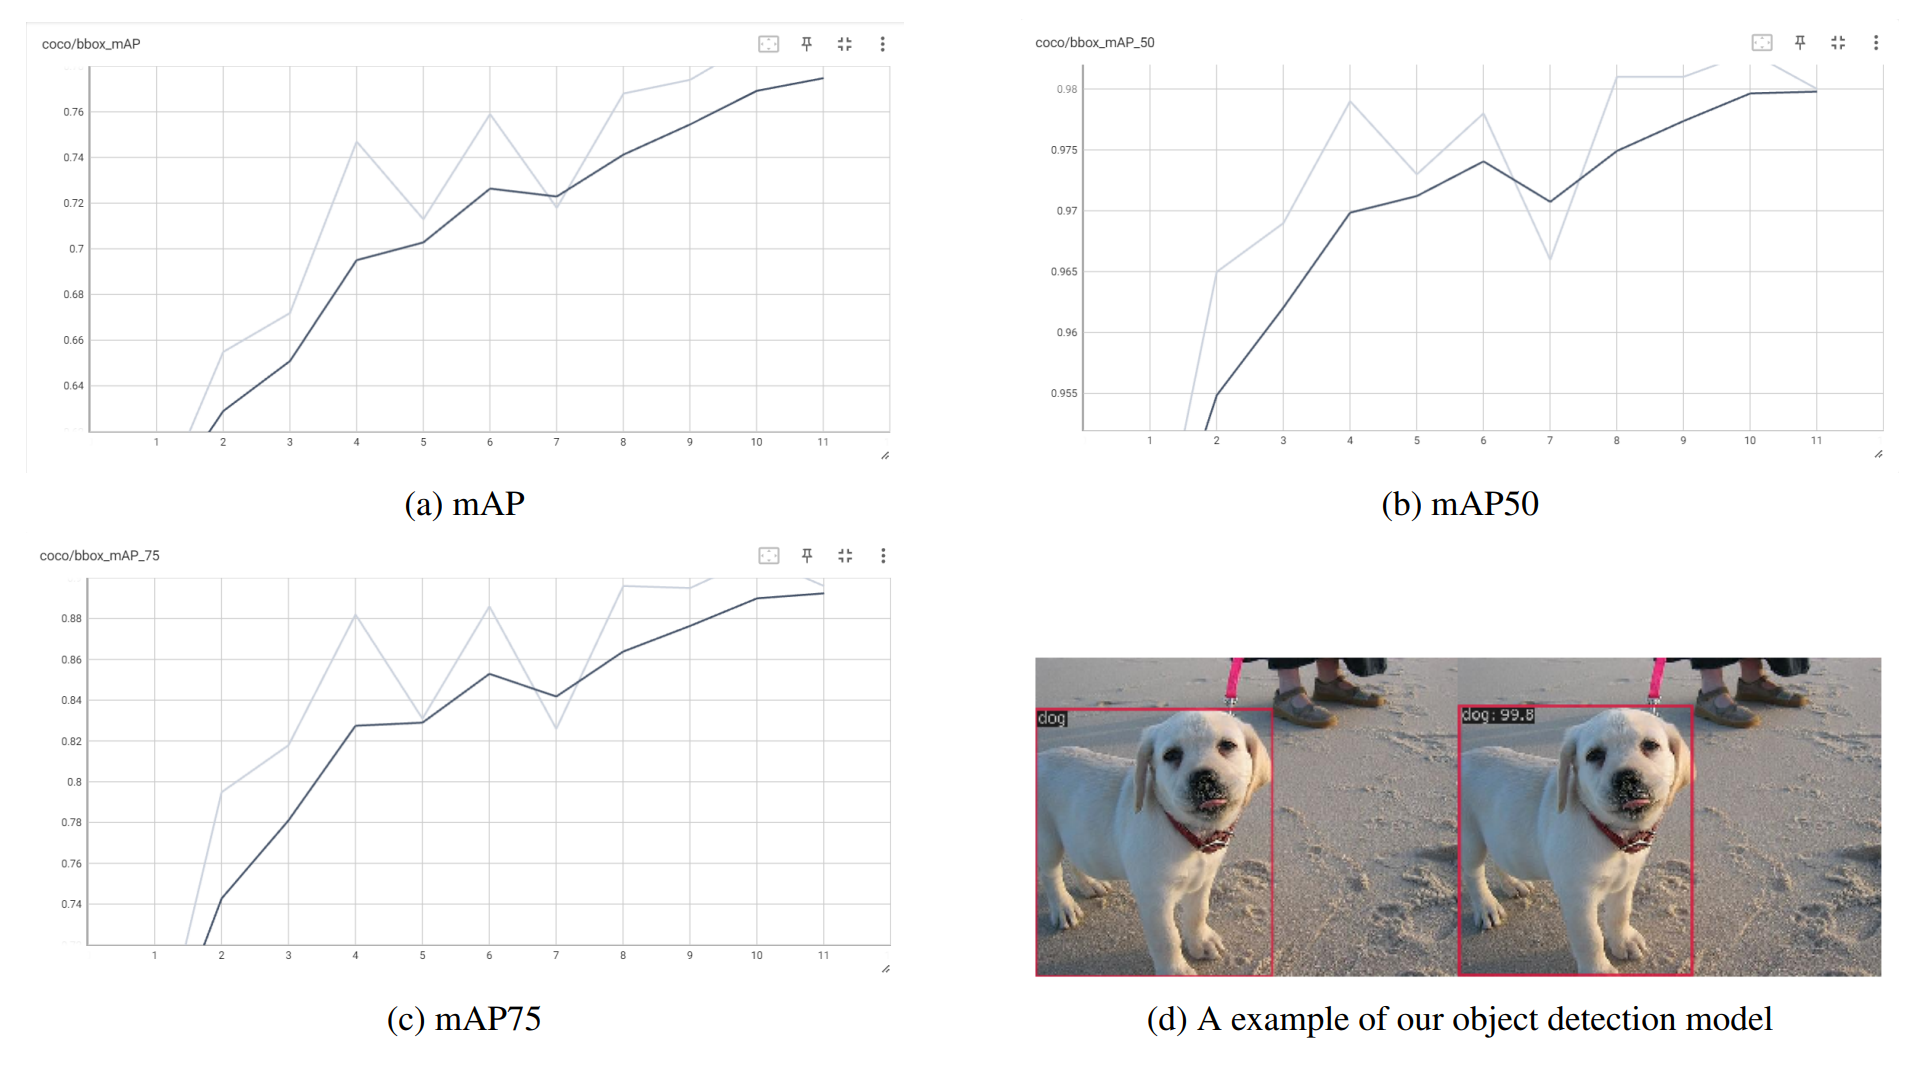
\includegraphics[width=12cm]{./img/pic1.png}
                \caption{Faster RCNN result}
            \end{figure}\par
        \end{frame}
        \begin{frame}
            \frametitle{Object Detection}
            We cropped each images using two different strategies:
            \begin{itemize}
                \item Crop as the predicted bboxes
                \item Find the nearest square shape to predicted bbox and crop it to square image
            \end{itemize}\par
            \begin{figure}[H]
                \centering
                \begin{minipage}[t]{0.48\textwidth}
                \centering
                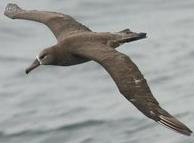
\includegraphics[width=4cm]{./img/bird1.png}
                \caption{Strategy 1}
                \end{minipage}
                \begin{minipage}[t]{0.48\textwidth}
                \centering
                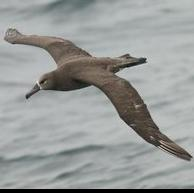
\includegraphics[width=4cm]{./img/bird2.png}
                \caption{Strategy 2}
                \end{minipage}
            \end{figure}\par
        \end{frame}
        \begin{frame}
            \frametitle{Object Detection}
            Question: Accuracy Rate decreases for both datasets after we use cropped images for training and testing.
            \begin{itemize}
                \item Each dataset dropped $1\sim 2$ percentage accuaracy rate after using cropped dataset
                \item No matter the cropping strategies
            \end{itemize}\par
        \end{frame}
    \section{Task 4: Synthetic Images}
        \begin{frame}
            \frametitle{Synthetic Images}
            Expected Pipeline:\par
            \begin{itemize}
                \item Getting bbox of trainset images from annotations 
                \item Getting bbox of testset images from inference results
                \item Cropping each image to bbox and resize it
                \item Generating more images from cropped images
                \item Training using images from trainset and generated iamges
            \end{itemize}
        \end{frame}
        \begin{frame}
            \frametitle{Synthetic Images}
            \begin{itemize}
                \item Using BigGAN-deep model, introduced by Brock et al. in Large Scale GAN Training for High Fidelity Natural Image Synthesis
                \item Use previously cropped images as input conditional datasets
                \item Using MMagic framework as training framework
                \item Unified resolution of images to 256x256
                \item Download BigGAN-deep model pretrained by ImageNet-1k dataset from Hugging Face
            \end{itemize}
        \end{frame}
        \begin{frame}
            \frametitle{Synthetic Images}
            We met problems in this task:\par
            \begin{itemize}
                \item Requires a lot of computing resources, limited us from trying different methods and comparing them (We trained this model using 4x Nvidia A100, costed $\sim 2$ days)
                \item Got unstable FID value during training process, not as the original paper claims (the original paper claims $~10$ FID value in different datasets)
                \item Our model generated images of poor quality, which have little value for extra training dataset
            \end{itemize}
        \end{frame}
        \begin{frame}
            \frametitle{Synthetic Images}
            \begin{figure}[H]
                \centering
                \begin{minipage}[t]{0.48\textwidth}
                \centering
                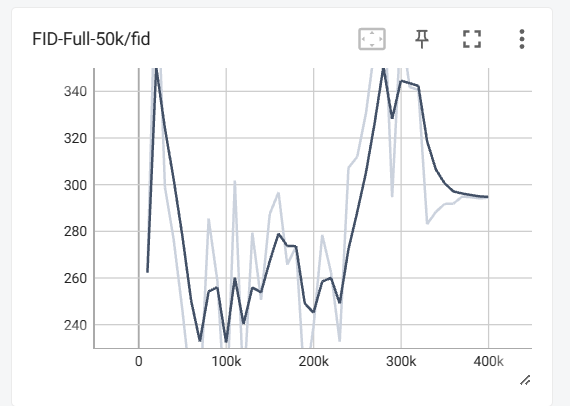
\includegraphics[width=5cm]{./img/pic2.png}
                \caption{FID value}
                \end{minipage}
                \begin{minipage}[t]{0.48\textwidth}
                \centering
                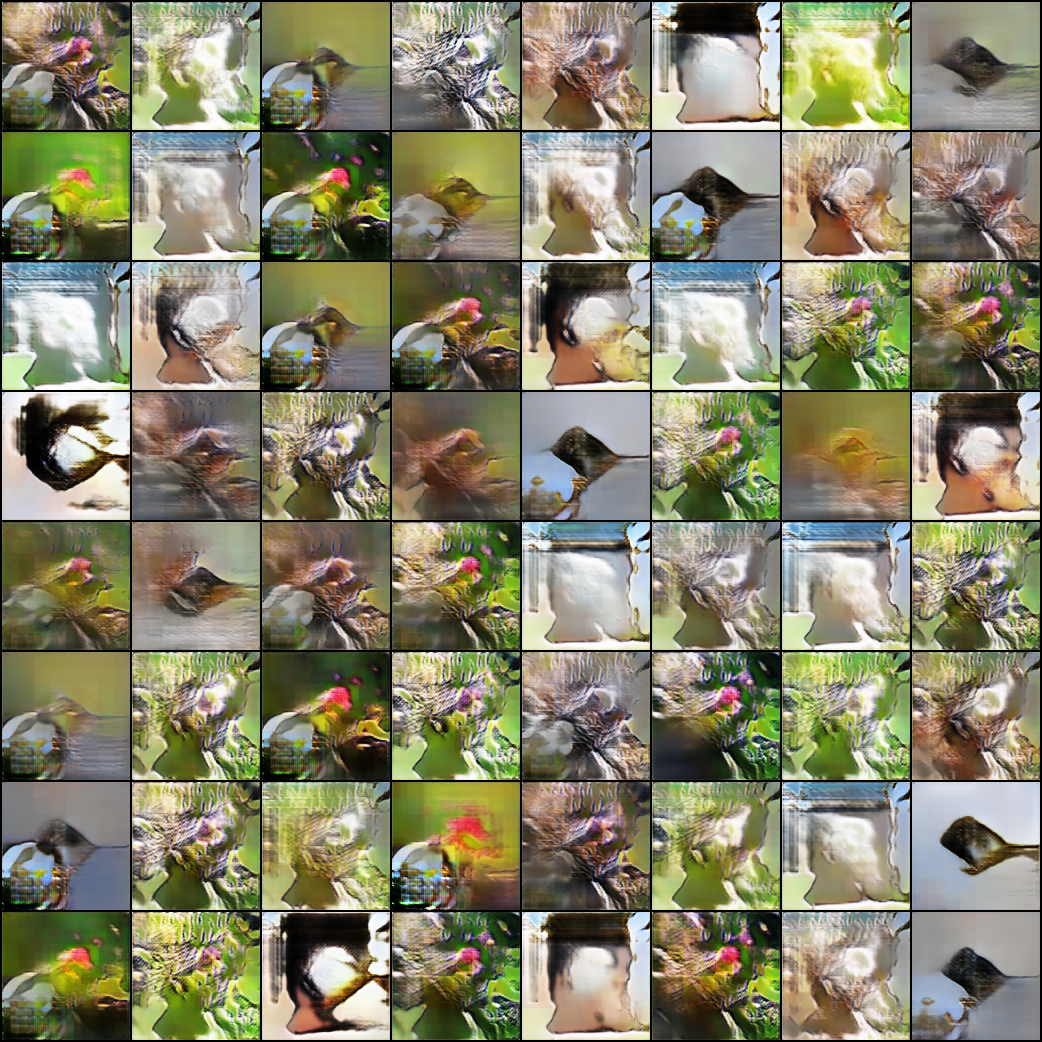
\includegraphics[width=5cm]{./img/pic3.png}
                \caption{Generated images}
                \end{minipage}
            \end{figure}\par
        \end{frame}
    \section{Task 5: Efficiently use ViT}
        \begin{frame}
            \frametitle{Efficiently use ViT}
            \begin{itemize}
                \item Explore different configurations (number of layers, number of attention heads, etc.)
                \item Consider using a hybrid model that combines both CNN and ViT. The CNN could be used to extract features from images, which can then be passed to the transformer for the classification task
                \item One of the biggest challenges with ViT is its demand for large amounts of data for training. Use transfer learning techniques, take a pretrained ViT model and fine-tune it.
            \end{itemize}\par
        \end{frame}
    \section{Task 6: Interpretation of the model}
        \begin{frame}
        \frametitle{Interpretation of the model}
        \begin{itemize}
            \item Use Class Activation Maps to visualize the regions of the image that were important for the model to make its prediction (based on the model's final convolutional layer)
            \item Visualize attention maps, allow us to see which patches of the image the model paid attention to when making its predictions
        \end{itemize}\par
        \end{frame}
    \section{Task 7: Robustness of the model}
        \begin{frame}
            \frametitle{Robustness of the model}
            \begin{itemize}
                \item Adversarial examples are inputs designed to fool the model by adding small perturbations that lead to incorrect predictions
                \item Defensive distillation: train a second model (the `student') to mimic the output of the first model (the `teacher')
            \end{itemize}\par
        \end{frame}
        \begin{frame}
            \frametitle{Robustness of the model}
            Using Projected Gradient Descent (PGD):
            \begin{itemize}
                \item Fast Gradient Sign Method (FGSM): Computing the gradient of the loss with respect to the input image and creating a new image that shifts each pixel by a small step in the direction of the gradient
                \item An iterative version of FGSM that applies FGSM multiple times with a small step size
                \item Projects the perturbed image back into an epsilon ball to ensure that the adversarial example does not go too far from the original image
            \end{itemize}\par
        \end{frame}
    \section{Discussions}
        \begin{frame}
            \frametitle{Discussions}
            \begin{itemize}
                \item Acknowledged from other groups, ONLY a conbination of Step 1\&2 can achieve 90+\% accuracy on two datasets, it is necessary to apply each steps to the model?
                \item Step 3 (Object Detection) lead to a drop in accuracy, how to explain this phenomenon?
                \item Step 4 (Synthetic Images) obviously can not improve the performance of the model, what is its usage?
                \item Robustness often comes at the cost of accuracy, need to make a trade-off between robustness and accuracy
                \item Use which mertics to measure the robustness of the model (F1 score, Certified Robustness, Lipschitz continuity, etc.)?
            \end{itemize}\par
        \end{frame}
    \begin{frame}
        \Huge{\centerline{Thank you!}}
    \end{frame}
\end{document}      